% !TEX root = illustrator_submission.tex

\section{Blend Modes}
\label{sec:blendmodes}

%Illustrator 9 first introduced and supported the PDF 1.4 transparency model \cite{TransparencyInPDF}.
%While intricate in its details, the basic
%model composites two colors, corresponding to an object ({\em source}) and backdrop ({\em destination}),
%to generate a single color result (typically the {\em new destination}) based on a palette of
%{\em blend mode} functions quantifying how the two input colors interact.

%\subsection{GPU Fixed-function Blending Insufficient}

\ifdefined\NOSHOW
\begin{figure}[tb]
  \center{\includegraphics[width=3.1in]{images/fixedfunction_blending.pdf}}
  \caption{\label{fig:fixedfunction-blending}
  Conventional fixed-function blending; just RGB data flow is shown but scalar alpha data path is similar..}
\end{figure}
\fi

%In the interest of hardware simplicity and performance,
%GPU hardware blending is generally implemented as a fixed-function unit capable of performing
%simple blending functions constructed with rudimentary math operations (i.e. multiplies, adds, min/max)
%%and minimal control logic.
%% as shown in Figure~\ref{fig:fixedfunction-blending}.
%The hardware blending functionality in OpenGL is sufficient to implement all the
%blend functions introduced by the compositing algebra of \cite{Porter:1984:CDI:800031.808606}.

\begin{figure}[tb]
  \center{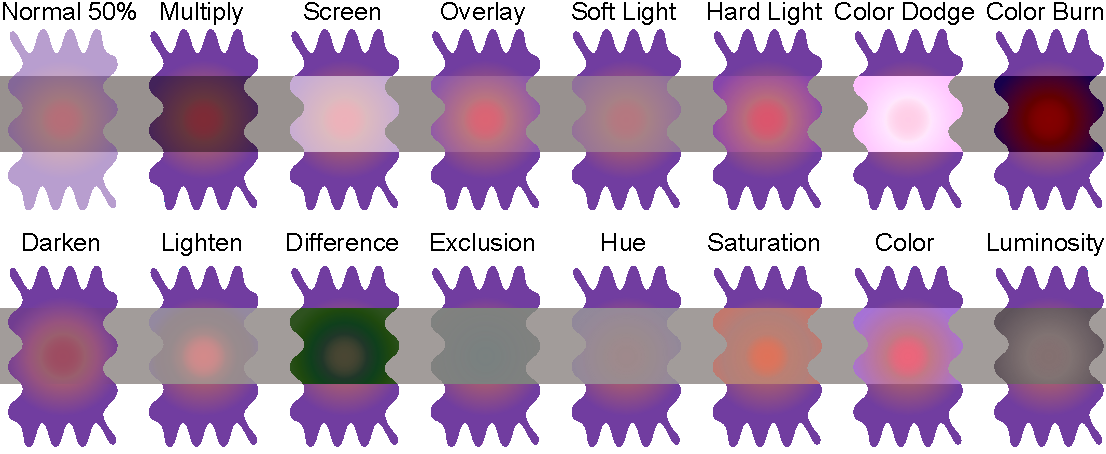
\includegraphics[width=3.3in]{images/blendmode_example.pdf}}
  \caption{\label{fig:blendmode-example} Example of all sixteen blend modes showing the interaction between a blob with an opacity gradient interacting with an overlapping rectangle with 90\% opacity.}
\end{figure}

Illustrator version 9 introduced a palette of sixteen blend modes.
These blend modes were subsequently incorporated into
the PDF standard's transparency model \cite{TransparencyInPDF}.

\subsection{GPU Blend Mode Support}

Of these modes
only two ({\em Normal} and {\em Screen}) are sufficiently simple that
they can be implemented with conventional OpenGL fixed-function blending.
Several of the advanced PDF
blend modes require intermediate numeric range exceeding the clamped [0,1] range
used in fixed-function GPU blending.
Some of the modes require simple ``if/then/else'' conditions, division, and square root operations.
To a hardware designer or anyone else first encountering these modes, they may seem {\em ad hoc} and  arbitrary,
but {\em HardLight}, {\em ColorDodge}, and the rest are firmly established in the vocabulary and training of digital artists \cite{HiddenPowerOfBlendModes}.  Figure~\ref{fig:blendmode-example} demonstrates their various effects.

\ifdefined\NOSHOW
Blending is the last step in the traditional GPU rendering pipeline and necessarily operates
at the {\em per-color sample} rasterization rate
(rather than {\em per-pixel} rate of multisample fragment shading)
and {\em after} stencil testing.
These are both important considerations
for Illustrator because blend modes and shading each specified independently and our
antialiased \NVpr/ usage relies on both 8x multisampling and stencil testing.
Even if blend modes
were extremely rare in real content,
the consequence of implementing a fallback to handle
the unsupported blend modes is very expensive, both in terms of poor performance and implementation
complexity.  \Illustrators/ 8x multisampling means {\em per-sample shading}
could run as slow as \nicefrac{1}{8}
%one-eighth
speed.
In practice, blend modes are sufficiently common in Illustrator artwork
to need efficient handling.
\fi

\ifdefined\NOSHOW
In anticipation of Adobe's requirements for blend mode support to GPU-accelerate
Illustrator,
%\footnote{Though blend modes are no longer limited to PDF and \Illustrator/.
%Flash \cite{SWF-File-Format}, SVG, and other
%compositing standards also incorporate blend modes (though the details
%vary).}
NVIDIA developed the OpenGL \NVbea/ extension \cite{NVbeaSpec}
and implemented its {\em coherent} flavor in their Tegra K1 and Maxwell GPUs.
Khronos subsequently standardized a multi-vendor subset \KHRbea/ \cite{KHRbeaSpec} to provide
the specific blend modes \Illustrator/, PDF, and SVG \cite{SVG-Compositing-Spec} require.
Either extension is sufficient for \Illustrators/ blending needs.

For NVIDIA GPUs that pre-date
this blend mode hardware functionality, the {\em incoherent} flavor of \NVbea/ and \KHRbea/ are
advertised and implemented through shader epilogues managed automatically
by the driver.  There is one explicit limitation of the non-coherent flavor: explicit {\em blend barrier} commands
must be used to ensure properly ordered blending.  However a special
exception is made for \NVpr/'s rendering operations because ``stencil,
then cover'' path rendering naturally lends itself to proper ordering.
For \Illustrator/, this means the same blend equation advanced programming interface
works on both older and newer NVIDIA GPUs without needing explicit blend barriers.
\fi

In anticipation of Adobe's requirements for blend mode support, NVIDIA
developed the OpenGL \NVbea/ extension \cite{NVbeaSpec} for advanced blending.  It
provides
all the blend modes needed by Illustrator, PDF, and SVG \cite{SVG-Compositing-Spec}.
The first-class {\em coherent} form of the extension
is implemented via hardware support in Tegra K1 and Maxwell
GPUs.
For older GPUs without hardware support for the coherent form,
the advanced blending functionality is exposed
through an {\em incoherent} form of the extension.
For the incoherent form, drivers 
are expected to implement the advanced blending as
a driver-generated epilogue to the application's fragment shader.
The incoherent form
requires the application to use
blend barrier commands to ensure proper blend ordering
to guard against read-modify-write hazards.
A special exception is made for \NVpr/
operations, since ``stencil, then cover'' path rendering naturally lends
itself to proper blending.

Khronos subsequently standardized OpenGL advanced blending functionality with the \KHRbea/
\cite{KHRbeaSpec} extension, also with coherent and incoherent forms.
AGM uses either OpenGL extension as available.

%\begin{figure}[tb]
%  \center{\includegraphics[width=2.8in]{images/iterated_blend.pdf}}
%  \caption{\label{fig:iterated-blend} Iterated blend hardware unit (right) as alternative to fixed-function blending (left).
%  %(see Figure~\ref{fig:fixedfunction-blending}).
%  }
%\end{figure}

\ifdefined\NOSHOW
\subsection{Alternative Hardware Approaches}
\label{sec:blendalternatives}

Recent hardware advances provide alternatives to introducing specific
blend modes.  Intel's {\tt INTEL\_fragment\_shader\_ordering}
\cite{INTELfsoSpec} (also supported by AMD GPUs) and NVIDIA's
{\tt NV\_fragment\_shader\_interlock} \cite{NVfsiSpec} provide
similer-but-different ``safely ordered'' mechanisms for the fragment
shaders to access the multisample framebuffer contents and perform arbitrary shader
computations within that shader.  If one tries to avoid the high cost of per-sample shading, 
the performance challenge for efficient per-pixel shading is the shader must perform
the blend mode math on each rasterized color sample within the pixel (times 8 in our case) but only
for color samples that pass the stencil test (relevant if color sample writes are done directly
by the shader rather than with conventional blending of the shader's color output).

While the viability of our GPU-acceleration effort and our contributions
(Section \ref{sec:contributions}) require some mechanism to handle all
PDF blend modes---and consideration of these alternatives is worthy of
investigation---their evaluation is outside the scope of the present
work.
\fi

\subsection{Premultiplied Alpha}
\label{sec:premultiplied}

One point of interest for GPU blending is how colors are represented.  Colors stored in GPU framebuffers and
textures must to be stored in pre-multiplied alpha form \cite{PreMultAlpha} for correct blending (including blend modes)
and texture filtering.  In contrast, the CPU-based AGM renderer stores color values with non-premultiplied alpha
consistent with the PDF specification.
